%% \chapter[htoc-titlei][hhead-titlei]{htitlei}
%% -----------------------------------------------------------------------------
\chapter[General introduction][General introduction]{General introduction}
\label{ch:intro}

This thesis describes the search for direct scalar top pair production, with
the decay of each stop via an $R$-parity-violating (RPV) interaction to a
charged lepton (electron or muon) and a $b$-quark, as shown in
Figure~\ref{fig:blstop_diagram}.
The analysis uses 20.3~\ifb of $\sqrt{s}=8~\TeV$ proton-proton collision data
collected with the \atlas\ detector at the Large Hadron Collider (LHC).

\begin{figure}[ht]
  \centering
  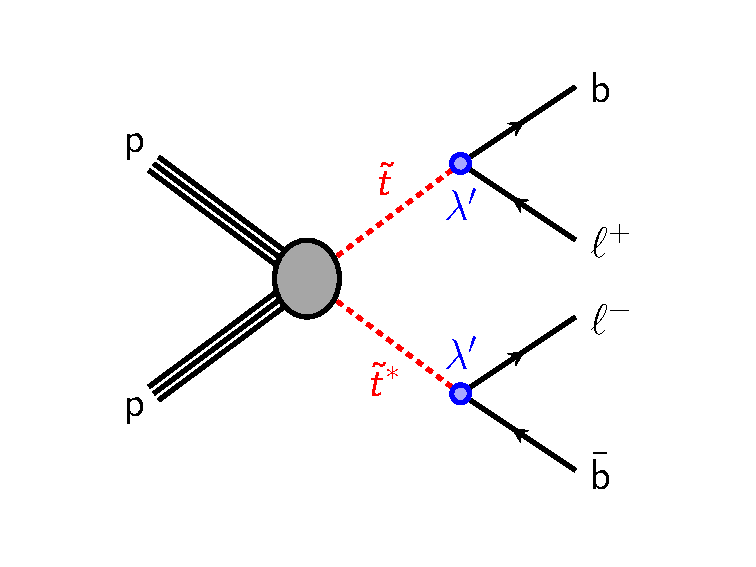
\includegraphics[width=0.60\textwidth]{figs/blstop/b_minus_l_stop_stop.pdf}
  \caption{Simplified model of pair production of scalar top quarks, with
    decay to a charged lepton and $b$-quark.
  }
  \label{fig:blstop_diagram}
\end{figure}


The experimental signature is two oppositely charged leptons and two identified
$b$-jets.
The analysis considers $eebb$, $e \mu bb$, and $\mu \mu bb$ final states.
Final states with $\tau$ leptons are not considered for this search.
The distinguishing features are two pairs, each of a lepton and a $b$-jet, with
a resonance in the invariant mass distribution of each pair.
In contrast to $R$-parity conserving searches, there is no significant missing
transverse momentum.

Previous searches for lepto-quarks at \atlas~\cite{ATLAS:2013oea,
ATLAS:2012aq, Aad:2011ch, Aad:2011uv} and
CMS~\cite{Khachatryan:2014ura, CMS:2014qpa, Chatrchyan:2012sv,
Chatrchyan:2012vza} have considered pair production of first, second,
and third generation lepto-quarks, but have not examined the signature
of a resonance in the invariant mass of an electron and a $b$-jet or a
muon and a $b$-jet.  The results of these searches have already been
interpreted to set limits on the stop mass and its decay
branching fractions in the $B-L$
model~\cite{Marshall:2014cwa, Marshall:2014kea}.

Chapter~\ref{ch:theory} describes the Standard Model (SM) of
particle physics and Supersymmetry, a popular extension to the SM.
The concept of $R$-parity, and the $B-L$ extension to the SM is also discussed
in this chapter.
Emphasis is placed on the phenomenology of this model.

Chapter~\ref{ch:lhc} introduces the LHC and \atlas, along with the triggering
system and event reconstruction.
Chapter~\ref{ch:mc} reviews the Monte Carlo event generator tools used to
estimate the detector response and efficiency to reconstruct the signal
process, and to predict the backgrounds from SM processes.

Chapters~\ref{ch:bl_stop} and~\ref{ch:results} describe the stop search.
Chapter~\ref{ch:bl_stop} reviews the search strategy and event selection.
Chapter~\ref{ch:results} presents the results and interpretation.
